% ---------------------------------------------------------------------------
% Capa: Escola Politécnica da USP, Engenharia de Computação
% Substitui a capa padrão do abntex2. O texto da versão (parcial ou completa)
% vem de \versaodocumento, definido em parcial.tex e final.tex.
% ---------------------------------------------------------------------------

% As cores azulpoli e cinzacapa vêm de config/preambulo.tex.

\renewcommand{\imprimircapa}{%
  \begin{capa}%
    \fontecapa
    \centering
    % --- Cabeçalho: selo da Poli, instituição, logotipo da USP ---
    \begin{minipage}[c]{0.2\textwidth}
      \centering
      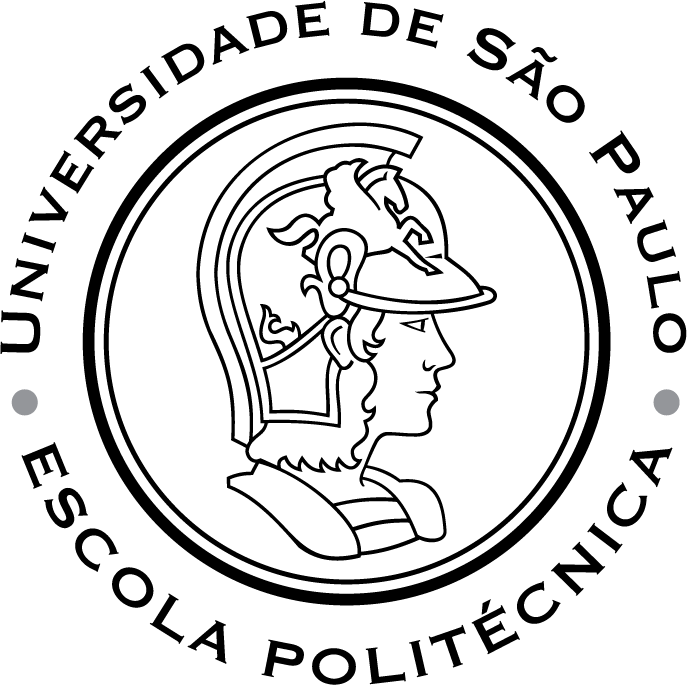
\includegraphics[height=2.9cm]{figuras/logo-poli}
    \end{minipage}%
    \hfill
    \begin{minipage}[c]{0.56\textwidth}
      \centering
      {\large\bfseries\MakeUppercase{Universidade de São Paulo}}\\[4pt]
      {\large\MakeUppercase{Escola Politécnica}}\\[8pt]
      {\small\color{cinzacapa}Departamento de Engenharia de Computação\\
       e Sistemas Digitais (PCS)}
    \end{minipage}%
    \hfill
    \begin{minipage}[c]{0.2\textwidth}
      \centering
      
\includegraphics[width=\linewidth]{figuras/logo-usp}
    \end{minipage}

    \vspace{0.6cm}
    {\color{azulpoli}\rule{\textwidth}{1.2pt}}

    \vfill

    % --- Título ---
    {\small\color{cinzacapa}\MakeUppercase{\curso}}\\[0.6cm]
    % 16,8 pt em vez do \LARGE (17,28 pt): no XeLaTeX não há expansão de fonte,
    % e o tamanho cheio quebrava o título em quatro linhas em vez de três.
    {\color{azulpoli}\fontsize{16.8}{22}\selectfont\bfseries\imprimirtitulo\par}
    \vspace{0.8cm}
    {\large\versaodocumento\par}

    \vfill

    % --- Autores ---
    \begin{tabular}{@{}l@{\hspace{1.2cm}}l@{}}
      \large\autorumnome   & \large\color{cinzacapa}NUSP \autorumnusp \\[6pt]
      \large\autordoisnome & \large\color{cinzacapa}NUSP \autordoisnusp
    \end{tabular}

    \vspace{1cm}
    {\normalsize Orientador: \imprimirorientador\par}

    \vfill

    {\color{azulpoli}\rule{\textwidth}{0.6pt}}\\[8pt]
    {\large\imprimirlocal\\[2pt] \imprimirdata\par}
  \end{capa}%
}
